\renewcommand{\thesection}{Basic Task}

\newcommand{\upa}{\mathlarger{\uparrow}}
\newcommand{\downa}{\mathlarger{\downarrow}}
\newcommand{\lefta}{\mathlarger{\leftarrow}}
\newcommand{\righta}{\mathlarger{\rightarrow}}

\section{Q Learning}

\subsection{Working Environment and State Transition and Reward Functions}

\begin{figure}[h]
	\begin{subfigure}{.49\textwidth}
		\centering
		\includegraphics[width=170pt,height=125pt,draft]{snow_puzzle_original.png}
		\caption{Original puzzle}
	\end{subfigure}
	\begin{subfigure}{.49\textwidth}
		\centering
		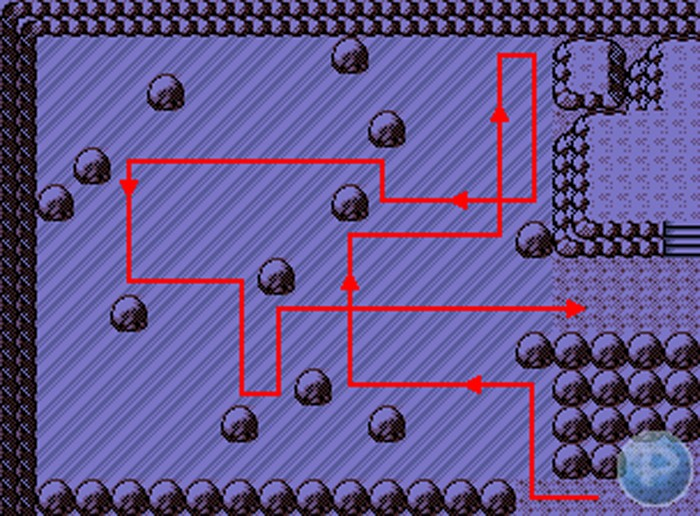
\includegraphics[height=125pt]{snow_2.png}
		\caption{Puzzle solution}
	\end{subfigure}
	\caption{An example of a Pokémon Ice puzzle}
\end{figure}

In this task we present a solver of \emph{Pokémon Ice Puzzles}, a kind of ice puzzle where the player starts at a certain position $s$ and has the objective to reach its objective $e$ in as few steps as possible.

At each turn, the player can do one of four movements: $\{\upa, \downa, \lefta, \righta\}$.
As the environment is ice, when the user walks in any direction is slips on the ice and keeps going on the same direction until hitting a rock or the edge.

\newcommand{\coor}[2]{\left\langle #1, #2 \right\rangle}
\newcommand{\yx}{\coor{y}{x}}
\newcommand{\obs}{\mathcal{O}}
\newcommand{\state}{\mathcal{S}}
\newcommand{\reward}{\mathcal{R}}
The state function $\state$, along with the transition and reward functions $\mathcal{T}$ and $\reward$ can be defined as the following, where $\obs_{\yx}$ is true if and only if there is an obstacle on position $\yx$.
\begin{gather*}
	\state = \yx \qquad \mathcal{D} \in \left\{ \upa, \downa, \lefta, \righta \right\} \\
	\begin{aligned}
		&T_{\yx}\left(\upa\right) &= \coor{t + 1}{x} &&&\text{where } \obs_{\coor{t}{x}} \wedge \neg \obs_{\coor{q}{x}} \forall q \in \left(t, y\right) \\
		&T_{\yx}\left(\downa\right) &= \coor{t - 1}{x} &&&\text{where } \obs_{\coor{t}{x}} \wedge \neg \obs_{\coor{q}{x}} \forall q \in \left(y, t\right) \\
		&T_{\yx}\left(\lefta\right) &= \coor{y}{t + 1} &&&\text{where } \obs_{\coor{y}{t}} \wedge \neg \obs_{\coor{y}{q}} \forall q \in \left(t, x\right) \\
		&T_{\yx}\left(\righta\right) &= \coor{y}{t - 1} &&&\text{where } \obs_{\coor{y}{t}} \wedge \neg \obs_{\coor{y}{q}} \forall q \in \left(x, y\right)
	\end{aligned} \\
	\reward(\yx) = \begin{cases}
		100 & \text{if } e = \yx \\
		0 & \text{otherwise}
	\end{cases}
\end{gather*}

\subsection{Q Function}

This transition function allows us to define an iterative $Q$ function, which should be used to find the objective $Q^\pi$ function.
\begin{gather*}
	s \in \mathcal{S} \qquad a \in \mathcal{D} \\
	\mathcal{Q}^{k + 1}(s, a) = \alpha \cdot \left( \reward( T( a, s ) ) + \gamma \cdot \max{Q^k(s, a)} \right) - Q^k(s, a)
\end{gather*}

\newpage{}
The next action $a$ is defined depending on the policy used.
\begin{description}
	\item[\textepsilon-Greedy Policy] \phantom{x}
		\begin{itemize}
			\item $\mathbb{P}(\varepsilon)$ \qquad Choose a random direction.
			\item $\mathbb{P}(1 - \varepsilon)$ \quad Greedily choose the $a$ with the highest $Q(s, a)$ with 
		\end{itemize}
\end{description}
